\section{Alex Pitcher Report - Rhys Tyers}

\margininbox{Alex Pitcher, 2012}{The Ghar Parau Foundation made two small Alex Pitcher awards to Rhys Tyers and Sam Page as a contribution to their first foreign caving expedition expenses. In return, they each wrote a personal account of their experiences, which we reproduce in this chapter.}{\award}

Having heard the other members of the club talk about little else  than the summer expedition to Slovenia since I joined the at the start of the academic year I was quite excited in the days before we left. My excitement was tempered slightly by the 24 hour minibus ride though which seemed to mostly consist of Germany in the dark. Arriving in the Alps was spectacular with breathtakingly huge mountains rising up on either side of the road and soon we were climbing into the mountains as we entered Italy and then Slovenia. The windy road down to \passage[town]{Tolmin} from the Italian border was an apt start to the expedition, thrilling and just a bit scary.


\begin{pagefigure}
\checkoddpage \ifoddpage \forcerectofloat \else \forceversofloat \fi
   \centering
\includegraphics[width = \textwidth]{2012/alex_pitcher/rhys/2012-08-16-2243-TharatornSupasiti-IMG_0245--orig.jpg}
\caption{The hike from \passage[town]{Tolminske Ravne} up to the \passage[mountain]{Migovec} plateau takes one along a path with numerous zigzags (or switchbacks) in the forest. \pic{Tharatorn Supasiti}} \label{forest path}
\end{pagefigure}


\passage[town]{Tolmin} itself was not at all what I expected. I had thought it would be old, rural and quiet. In fact it was extremely modern with shops and restaurants and was surprisingly busy for such a small place. And then we arrived at our \passage[town]{Tolmin} base, \passage{Tetley’s} (James Hooper’s) flat. I was told that you could see \passage[mountain]{Migovec} from the flat but today it was shrouded in ominous clouds. The next day the clouds had not cleared. We drove up another windy road up to \passage[town]{Ravne}, the clouds swirling and darkening overhead. We unpacked our food and equipment into the barn that serves as the storage unit for the expo and prepared ourselves for the walk up. As we got our bags on our backs it started to rain, it was as though the entire cloud had fallen at once but, undaunted, we set off. The walk was more difficult than I had thought it would be. I was tired almost immediately and every zig or zag of the path I had to stop to rest.

Four hours later we reached the camp, a ‘plateau’ consisting of the flattest land available on the mountain next to a shakehole with a rock bridge. Home for the next five weeks. The Bivi, the communal area in the shakehole under the rock bridge, whilst initially strange was incredibly easy to find a place in. The tent I was sharing with Sam and Oli was also comfortable and had the same ‘nearly waterproof’ feel of the Bivi.

My first trip into \passage{Vrtnarija} (the cave system we were exploring) was with Jarv, we were going to rig the cave down to the underground camp. Despite the novelty of being on a mountain I immediately felt comfortable as I completed the familiar wriggling and stretching into my caving kit. Following Jarv was tiring despite the fact that I was not actually doing any of the rigging but soon I had descended beyond the depth of a normal Yorkshire cave and was still descending. Past \passage{Laurel}, \passage{Piston}, \passage{Pico}, \passage{Tessellator}; all names I had heard over the year that now had a physical shape to them. Half way down \passage{Space Odyssey} and about half way to camp Jarv decided to turn back and leave the rest of the rigging for someone else. The realisation that I now had 250 m of ascent ahead of me was daunting but there was only one way out. An age later we emerged onto the surface into the blackness of night. It could’ve been just another chamber apart from the grass and stars gave it away.

My second trip was with Tetley. We were the first team to go down after the camp had been set up so we arrived to a mostly tidy camp. We had decided to spend a night at camp before doing any pushing so we set about making dinner. Cheesey soupy fishy smash, a Tetley specialty and soon a staple of my diet. The next day we set off. The destination: \passage{Salvation}, 700m below the surface and a long way from camp. Across \passage{Zimmer}, down the loose, muddy slope of \passage{Cheetah}, down \passage{Wonderland}, across \passage{Red Baron Chamber}, up to the \passage{Throne Room}, and storm down \passage{Amazing Grace} and \passage{Magic Dragon}. Then \passage{Stuck in Paradise}. The pitch was like nothing else I have seen -- horrifically muddy, awkward rebelays, tight ropes caught round flakes, \bignote{all punctuated by Tetley’s giggles}. Once down it was a simple hour long crawl through \passage{Penitence} and then stooping through \passage{Salvation} to the pushing front.

\margininbox{Brave New World}{
     \begin{itemize}
    \item James "Tetley" Hooper
    \item Rhys Tyers
    \end{itemize}}{\explo}

A draughting squeeze. It was apparent that without some hammering and digging we weren’t getting through. After much work, mostly by Tetley, we broke through into a small chamber which led up through to a boulder choke above us. Whilst digging through this Tetley became trapped by a small boulder that fell on his waist. To him it apparently seemed like the end, he was to spend his last moments alive slowly starving to death at the bottom of this cave. To me, because I could actually see the small rock lying on him, it seemed like he was being lazy and not bothering to push it off. \bignote{I refused his attempts to bequeath me his tobacco} and instead tried to get the rock off him. To be fair to him it was quite heavy and with much effort Tetley managed to free himself. We continued past the boulder choke to another small chamber and then to a flat out, upwards crawl. This led to a dodgy free climb up some large boulders which then led to an underdeveloped streamway with a tiny trickle of water in it. It was here that we decided to stop and head back out. We said goodbye to the newly named ‘\passage{Brave New World}’ and began the long journey back to camp. This took six hours and at the time it was one of the hardest things I had physically done.

\begin{pagefigure}
\checkoddpage \ifoddpage \forcerectofloat \else \forceversofloat \fi
   \centering
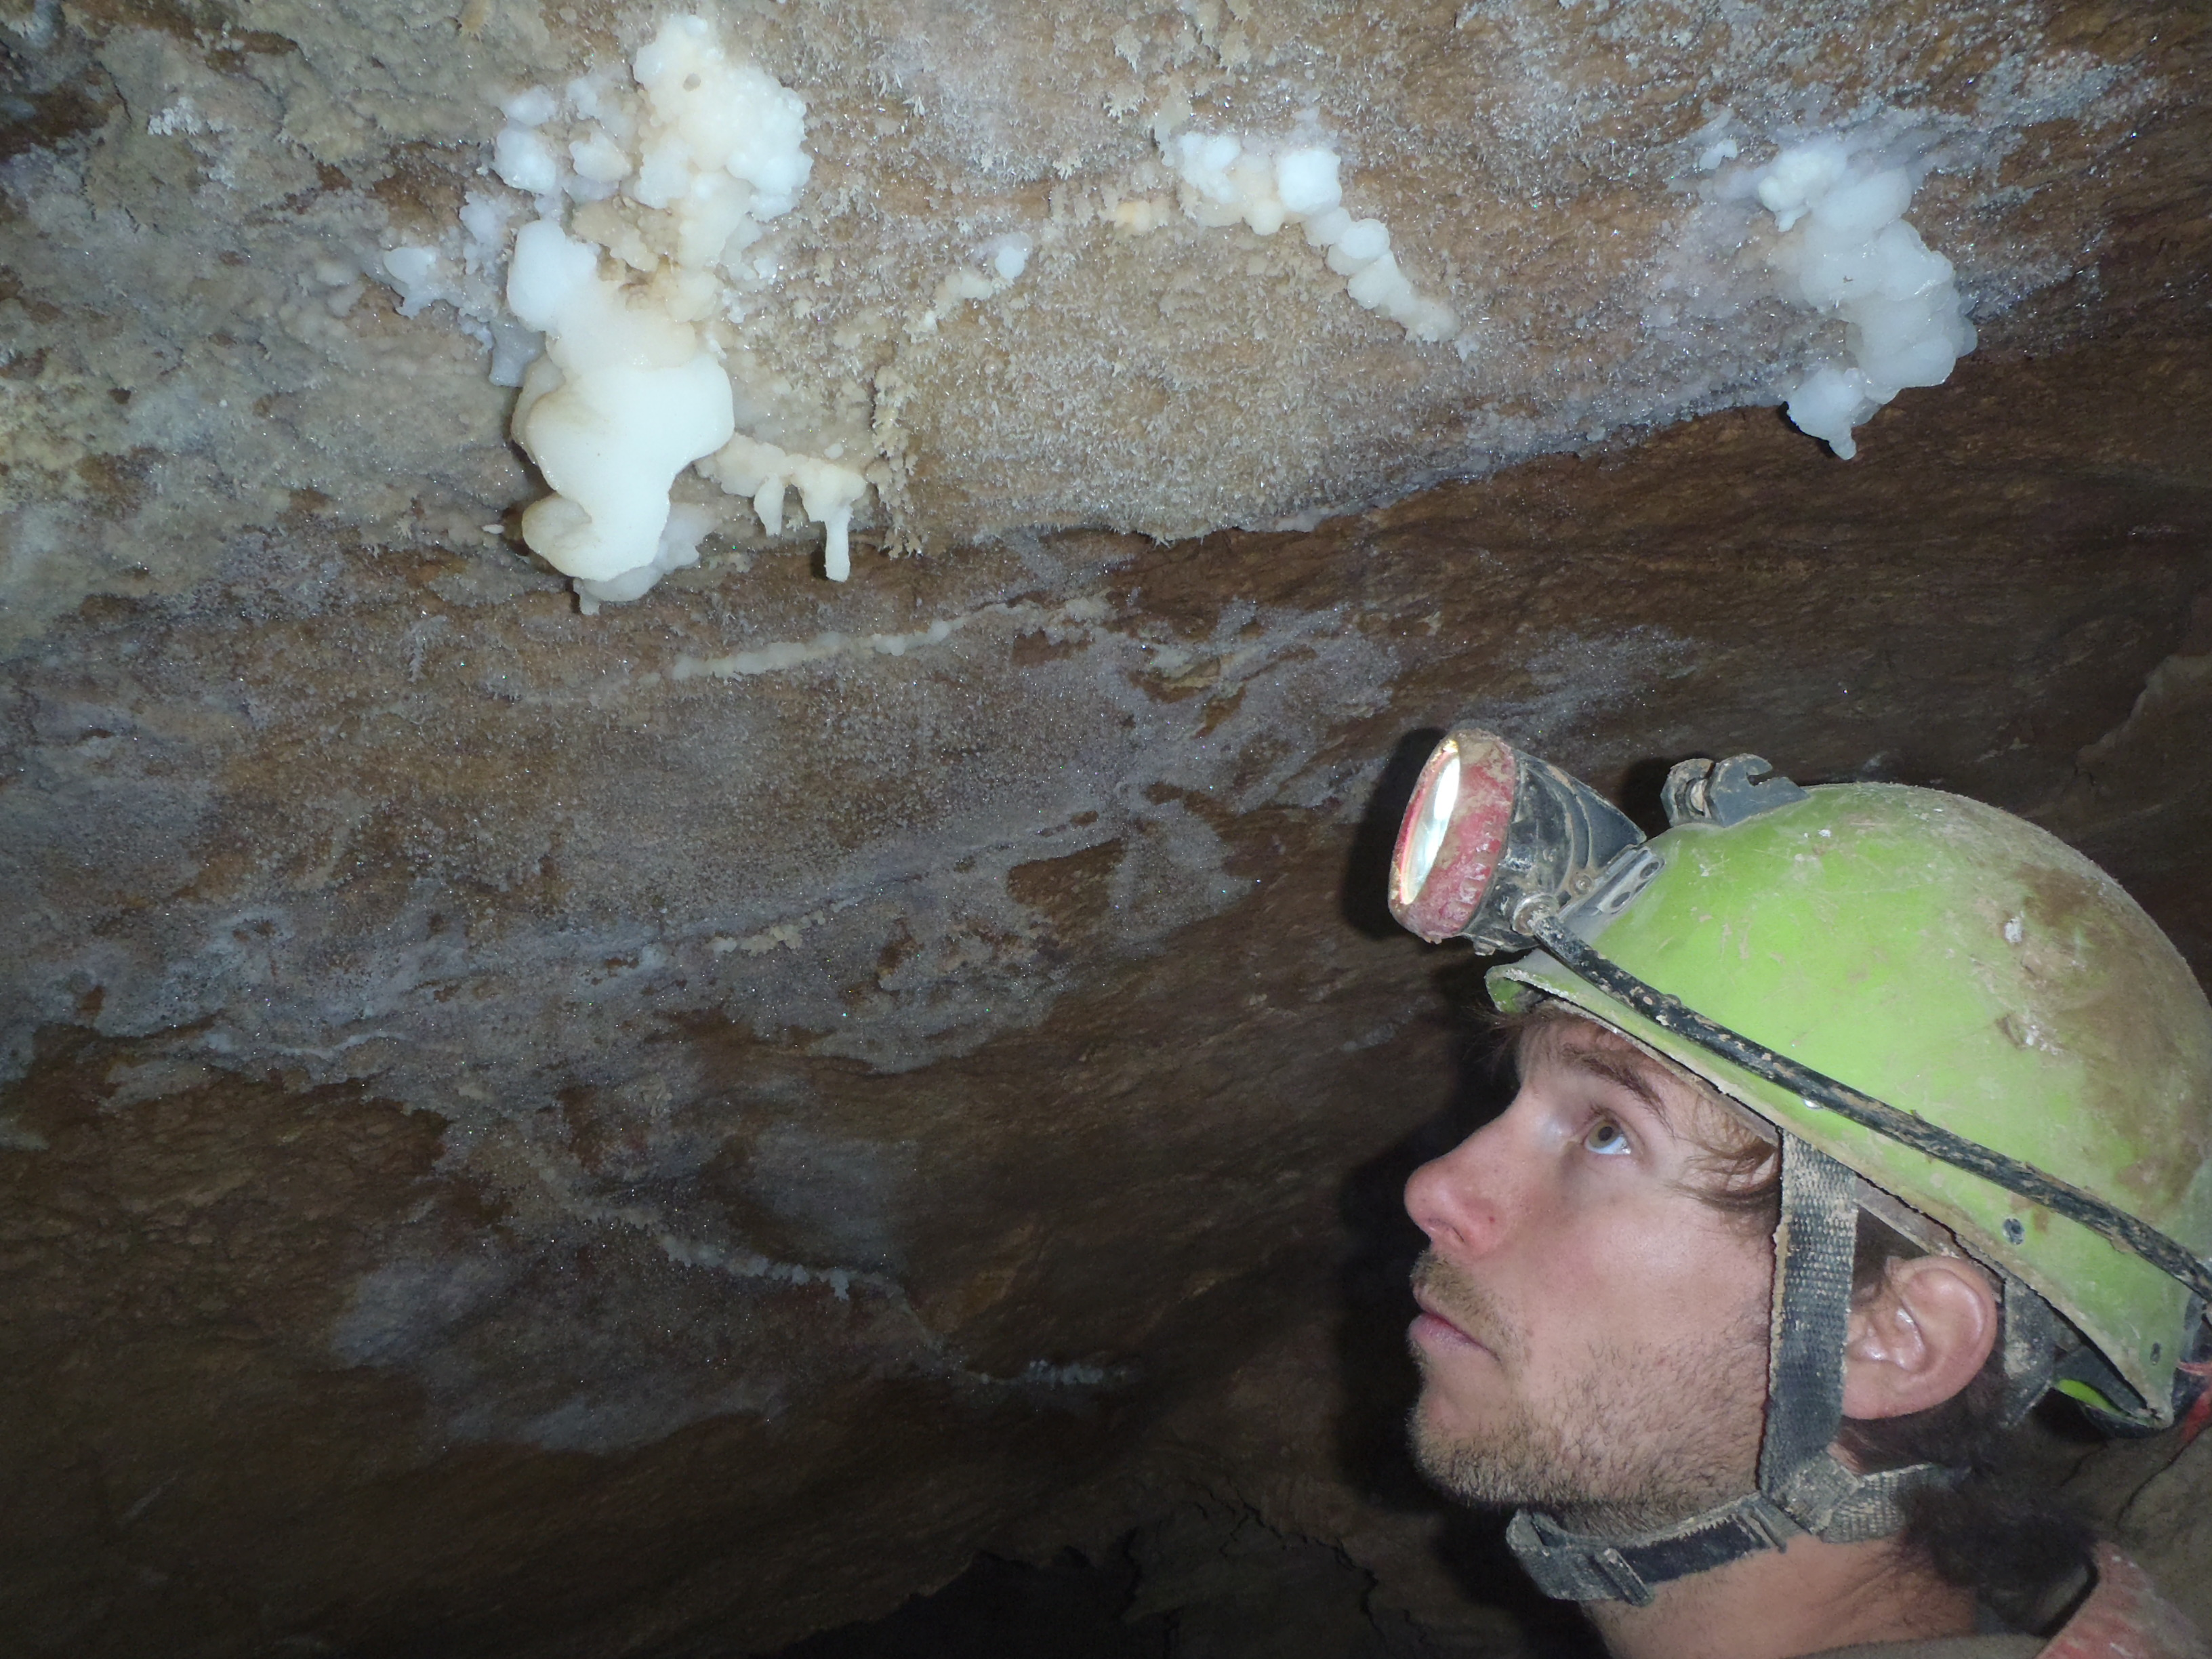
\includegraphics[width = \textwidth]{2012/alex_pitcher/rhys/2012-08-03-0358-Maver-P8030150--brave new world--orig.jpg}
\caption{Gergely Ambrus looking at formations on the ceiling of \passage{Brave New World}. \pic{Nejc Maver}} \label{brave new world}
\end{pagefigure}

\margininbox{Xanadu}{
     \begin{itemize}
    \item James "Tetley" Hooper
    \item Rhys Tyers
    \end{itemize}}{\explo}

Luckily for us no-one had booked the next slots at camp so we were able to sleep for 16 hours and wake up thoroughly confused as to what day it was. Feeling that we had accomplished some impressive pushing already Tetley and I opted for an easy day. We were to have a look at a little dig that Tetley had found two years previously. We set off and five minutes later we arrived. Tetley was not confident that the dig went anywhere but almost immediately upon crawling into it he decided that it did in fact go into a small rift. After moving up and down on various levels in the rift, going back to camp to get bolting kits (what a luxury) and bolting down the scarier climb (incidentally my first bolt in the cave), we got down to a beautiful stream. This was certainly very different to the day before. Here the pushing was easy and the cave pretty. However the stream sumped in one direction and led into a tight, waterfall in the other (which we left as a lead for someone else). Tetley, using what I can only assume was some sort of sixth sense for caving, decided that there was a sump bypass somewhere. There was, a little high up crawl/traverse over a rather dangerous drop. I’m quite proud of myself for spotting it. This led into the old streamway. There was a strong draught and it was cold. The stream way was perhaps half a metre high and pristinely beautiful. As we crawled into it I realised that the sand was a thin layer covering thick, sticky mud. This meant that I would probably be the first and last person to see the tube in its prettier form. We pushed until we got to a puddle. Showing grit and determination we decided to leave the cold, wet crawling for someone else and surveyed out of ‘\passage{Xanadu}’.

\tweet{11:43AM Jul 23, 2012}{SALVATION pushed through a BRAVE NEW WORLD of boulder chokes.No stream - howling draught!THRONE ROOM has two drill bolted leads(HOT PANTS).}

After another night at camp it was time to head out. This was hard and took several hours. Employing the Tetley method of stopping for chocolate at the top of \passage{Fistful of Tolars} and then again at \passage{Tessellator} does help to break the journey up. And of course at the top of \passage{Tessellator}, you’re practically out of the cave. I think something I will never forget, as we emerged into glorious sunshine, is the smell. It was like I could smell every flower and plant on the mountain. Three (maybe four) days well spent I think.

My second trip was unusual in that our team consisted of 4 people rather than the usual two. Gergely, Clare, Kate and me. After a almost familiar trip to camp, we dropped off our supplies and headed for \passage{Lost Miles}. At the bottom of \passage{Stuck in Paradise} we had a break. We had brought food and meths so we were able to make some minestrone soup. Kate offered about half of the soup to the caving gods by spilling it on the floor but what was left was really nice. After that we got to the pushing front at the end of \passage{Lost Miles} where there was a boulder choke to push through (this expedition seems to have a theme going). 

\margininbox{Minestrone \& Atlantis}{
     \begin{itemize}
    \item Gergely Ambrus
    \item Kate Smith
    \item Clare Tan
    \item Rhys Tyers
    \end{itemize}}{\explo}

Clare and Gergely hammered their way through it whilst Kate and I (mostly Kate) tried to remember the words to ‘There’s a Hole in my Bucket’. Once we got past the boulder choke we discovered what every caver hopes for, hundreds of metres of easy walking (or stooping passage). The passage split into two and we explored both.

‘\passage{Minestrone}’ had a few crawls and was generally stooping passage between little chamber. The other passage was mostly walking and at the end we discovered the first major cave formations for this cave system. Stalactites, stalagmites and straws lined the walls. Because of this treasure of the deep, we called this part ‘\passage{Atlantis}’.

The next day Gergely and I went to push a lead off \passage{Minotaur Rift}. This was supposed to be an easier trip, being only an hour from camp. It turned out to be a long crawling section that required a lot of digging, all while sharp rocks from the ceiling fell on us. After a lot of crawling and digging, I was ready to give up and leave it for someone else but Gergely wanted to look round the corner. There just metres from where I wanted to quit was a chamber with a stream in and just a short crawl from that there was a huge rift. We then surveyed out, calling the new passage ‘\passage{Guillotine}’.

My third trip was again with Tetley, who after flying back to \passage[town]{London} upon discovering that I was caving with Gergely flew back when he heard what we had found. We had decided to go back to the end of \passage{Brave New World} and continue pushing there. We had been told there was another boulder choke to get through and it didn’t look good but we weren’t deterred. Now that I had been a few times we made it past \passage{Stuck in Paradise} and to \passage{Brave New World} relatively quickly. The crawl we had left it at last time was indeed blocked by large boulders and Tetley went in to have a look. As I lay behind Tetley I stared at an opening in the rock on the left, then Tetley called back ‘Is there a way through on the left?’, ‘Funny you should say that’ I said.

\margininbox{Invictus}{
     \begin{itemize}
    \item James "Tetley" Hooper
    \item Rhys Tyers
    \end{itemize}}{\explo}

I went into it and decided we could get through it with some hammering so I left to get the hammer, which we had left at the start of the crawl. When I got back, Tetley was through having decided to ‘go for it’. Hammering didn’t prove to be that useful anyway and we left it as a fairly awkward double squeeze. Now beyond the boulders we were in a wide, low roofed passage and after some searching we found the way on. It lead into amazing walking passage with piles of sand as high as a person on either side, I had never seen anything like it. Walking along this we started to hear the sounds of water, a waterfall perhaps? We decided to go back and survey to here, hoping our curiosity would help keep us motivated. When we did peek round the corner the passage broke into a shaft, about halfway up. There was a waterfall flowing down the shaft We looked around and decided there was no way on without descending the shaft. We would need rope, oh well, something for next year, we thought.

\margininbox{Yorkshire}{
     \begin{itemize}
    \item James "Tetley" Hooper
    \item Rhys Tyers
    \end{itemize}}{\explo}

The next day, after a mere 10 hours sleep we decided to go and push somewhere close to camp. The place was called ‘\passage{Yorkshire}’, only 10 minutes from camp. An awkward crawl leads to a surprisingly large pitch. At the bottom Tetley and I searched for a way on, eventually deciding that it must be following the stream down a small pitch. We assumed that Ollie and Thara must have done a dodgy free climb down but as we had the kit we bolted down. At the bottom there was a small narrow crack in the wall which we attempted to squeeze down but decided to exit. A horrible wet immature streamway was too much for us, we probably had underestimated how tired we were from our previous trip. So with still lots of time left in the day (or night, time isn’t normal in the cave) we decided to do a trip to visit the old camp at a place called \passage{Cactus Junction}. We went down a pitch called \passage{Big Rock Candy Mountain} which is a truly awesome pitch. The old camp was interesting and very cold (aptly named ‘\passage{The Fridge}’).

Those were my pushing trips but I also did a couple tourist trips through \passage{System Migovec}. That was incredible and I’m very glad I did it. The difference between the (at the time) two systems was astonishing. Where \passage{Gardener's World} is generally quite small, and you’re lucky to get walking passage, \passage{Sys Mig} is enormous and it's occasionally nice to see your light reaching the opposite wall. The chamber at the end of \passage{Exhibition Road} in particular is one of the most impressive things I have ever seen.


\begin{figure}
\checkoddpage \ifoddpage \forcerectofloat \else \forceversofloat \fi
\centering
 \frame{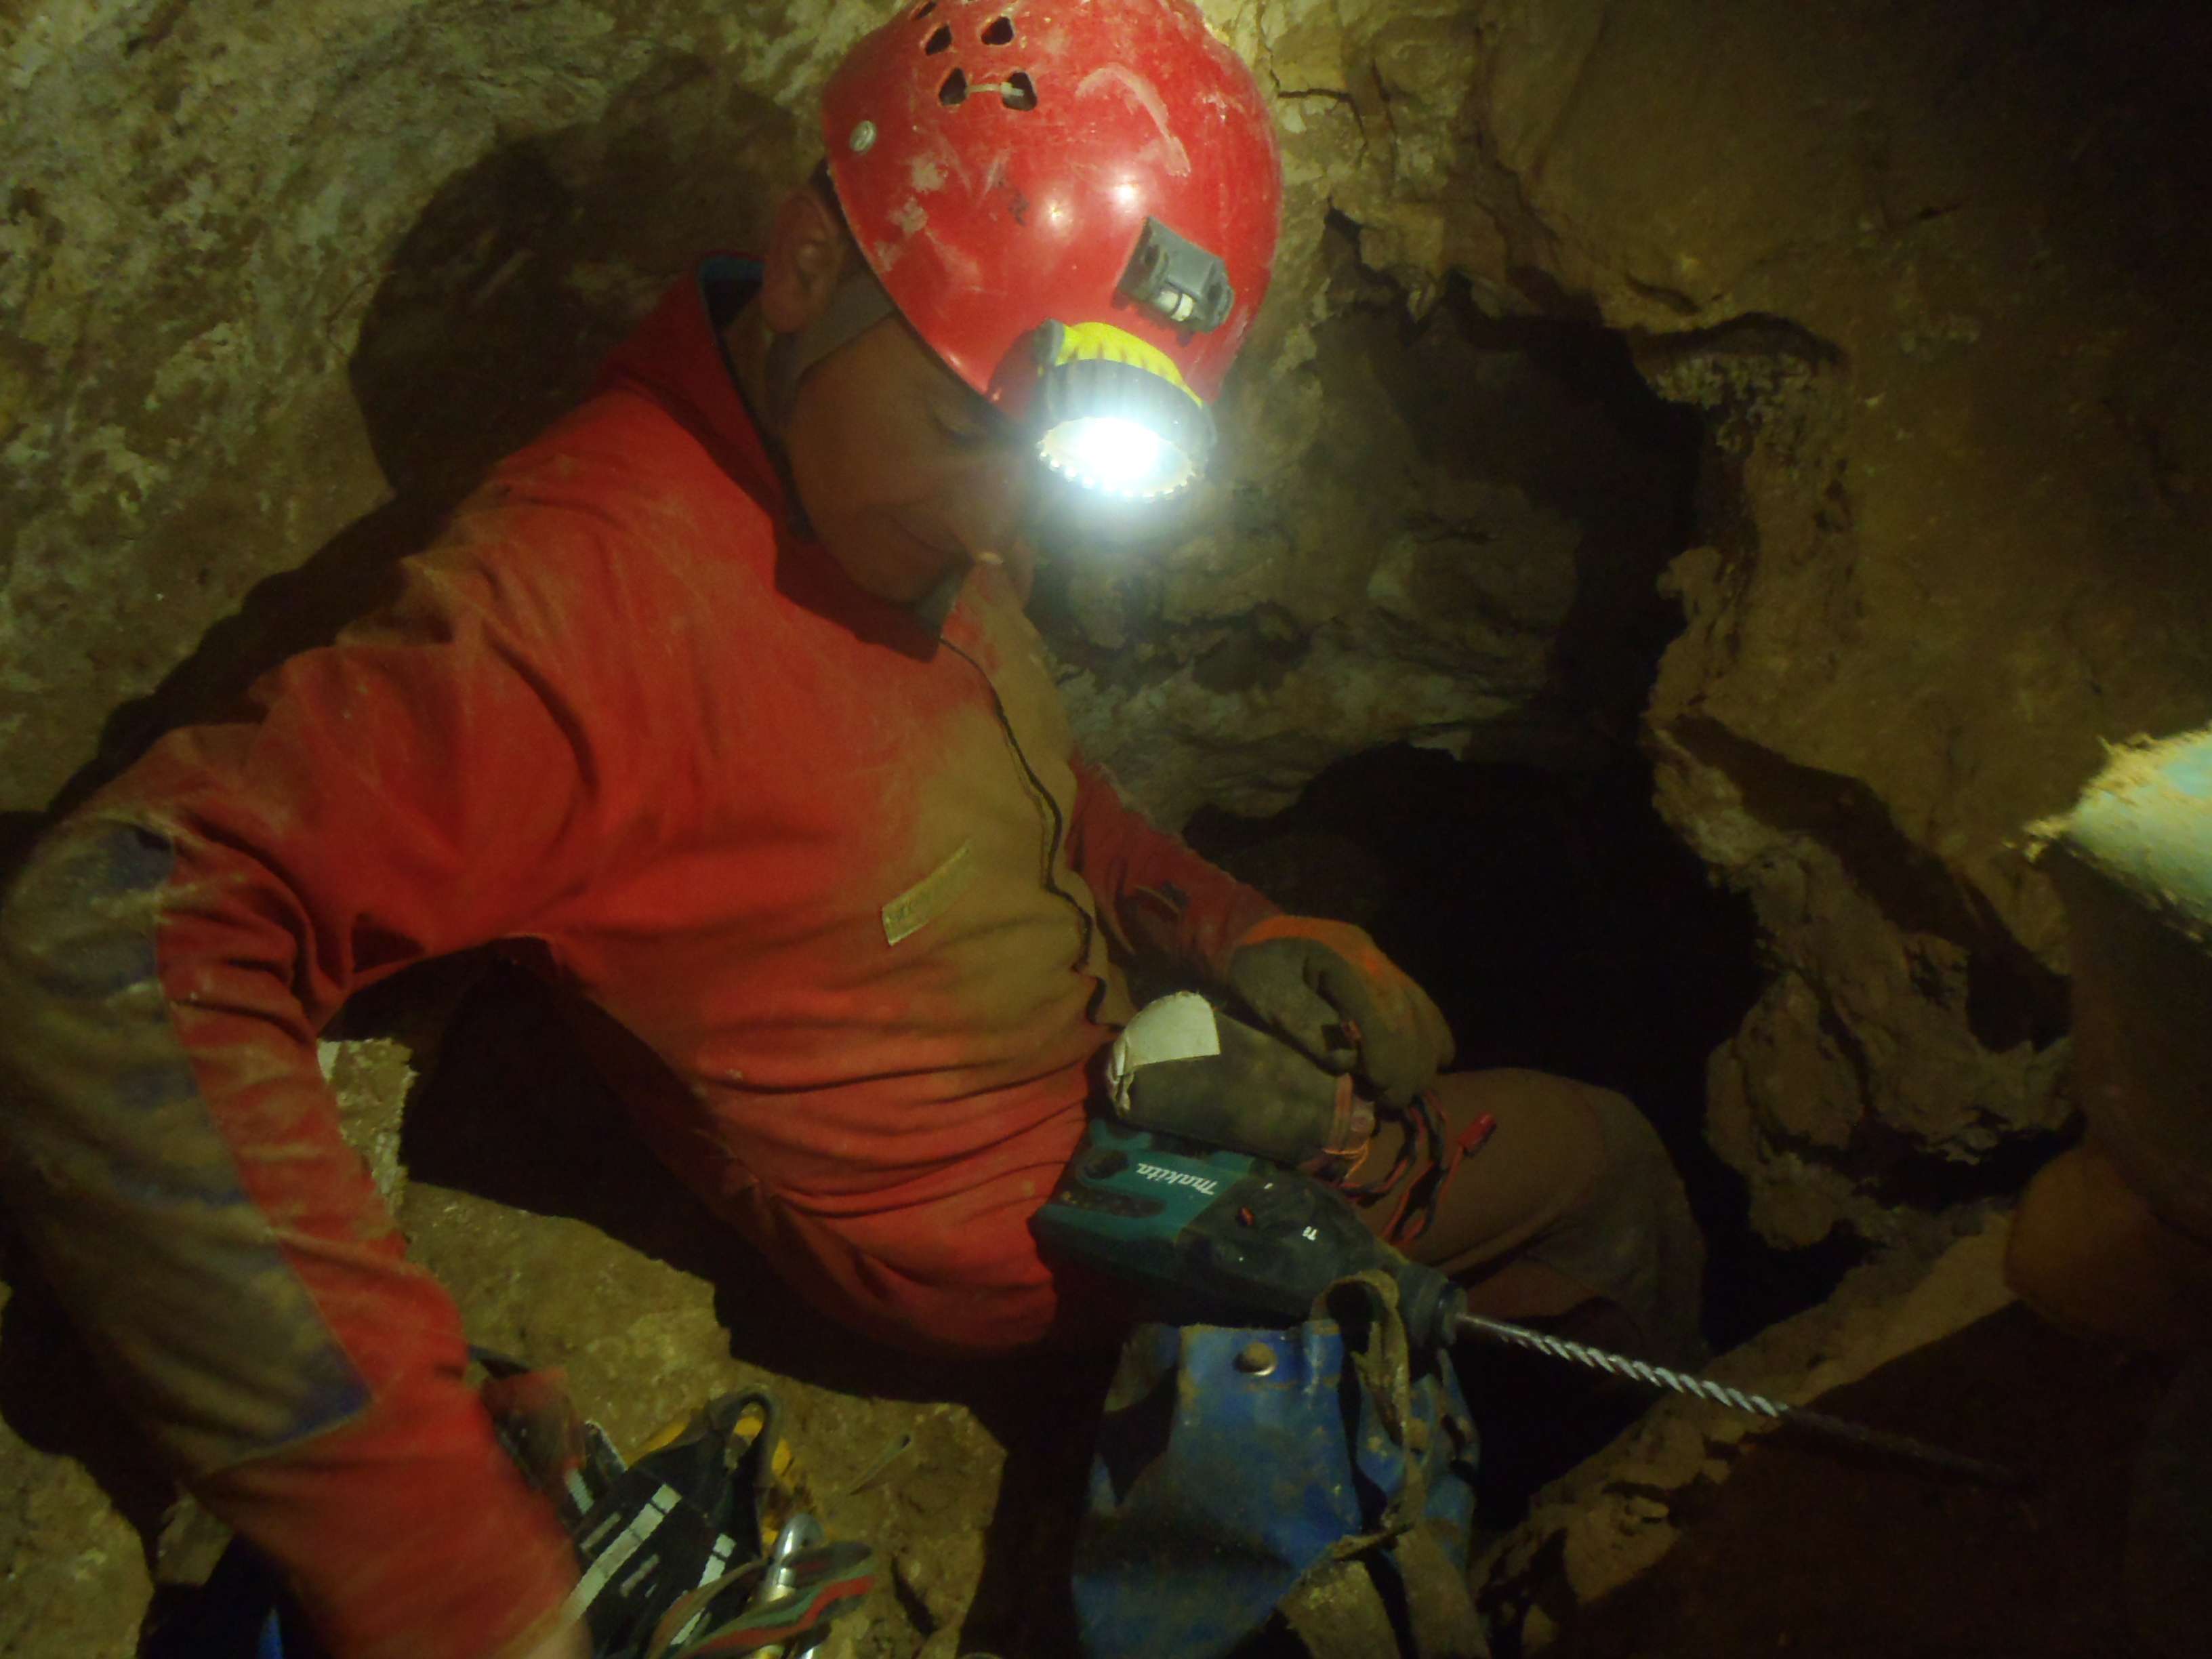
\includegraphics[width=\linewidth]{2012/alex_pitcher/rhys/2012-07-31-1321-IztokMozir-P7310667--orig.jpg}} 
 \caption{Fratnik and his drill seeking the connection between \passage{M2} and \passage{Vrtnarija}. \pic{Iztok Možir}}
 \label{m2 drill}
\end{figure}


\margininbox{Wizard of Oz}{
     \begin{itemize}
    \item Andrej Fratnk
    \item James "Tetley" Hooper
    \item Tim Osborne
    \item Clare Tan
    \item Rhys Tyers
    \end{itemize}}{\explo}

My other notable trip was the last ever ‘Super Action’ trip. These trips have been occurring regularly throughout the last year to attempt to connect the two cave systems, \passage{Gardener's World} and \passage{System Migovec}. The aim is to go to the closest point between the two cave systems and find a way through. This is slowed by the fact that the passage they are following regularly falls below human sized. The trip down was difficult and although I did say that \passage{Sys Mig} was big, the way down to the pushing front is not at all. The team consisted of Fratnik, Tim, Clare, Tetley and me. For me the day was fairly easy. I mostly watched Fratnik and Clare scurry in and out of a small crawl. Unfortunately, after much work, we did not make a connection, we may have even killed the lead. So we headed out. This was probably one of the hardest journeys I had made. I mostly attribute this to the drill I had to carry out. There wasn’t a single point on the way out that I didn’t feel exhausted, but make it out I did.

The last trip was the derig. Around 10 of us went down to camp to pack it all away into tackle sacks and carry it out. The way down was \bignote{fast and fun as I didn’t have a bag}. We would meet Gergely and Karin at camp, they had been the last team to do any pushing and would still be at camp. When I got to the bottom, I met Jonny who was packing rope and metal work in by \passage{Zimmer}. As I got to him he said ‘Gergely and Karin had good trip, they made the cave 30m deeper’.

I thought about this for a second, I remembered people saying that the water table stopped us from going any deeper. Maybe Jonny has gone mad and I should prussik away immediately, I thought. He did have a crazy look in his eye. And then it hit me. The entrances to \passage{Sys Mig} were higher than the \passage{Gardener’s World} entrance, they had made the connection! It was like a film, on the last pushing trip we had achieved this major goal.

\begin{marginfigure}
\checkoddpage \ifoddpage \forcerectofloat \else \forceversofloat \fi
\centering
 \frame{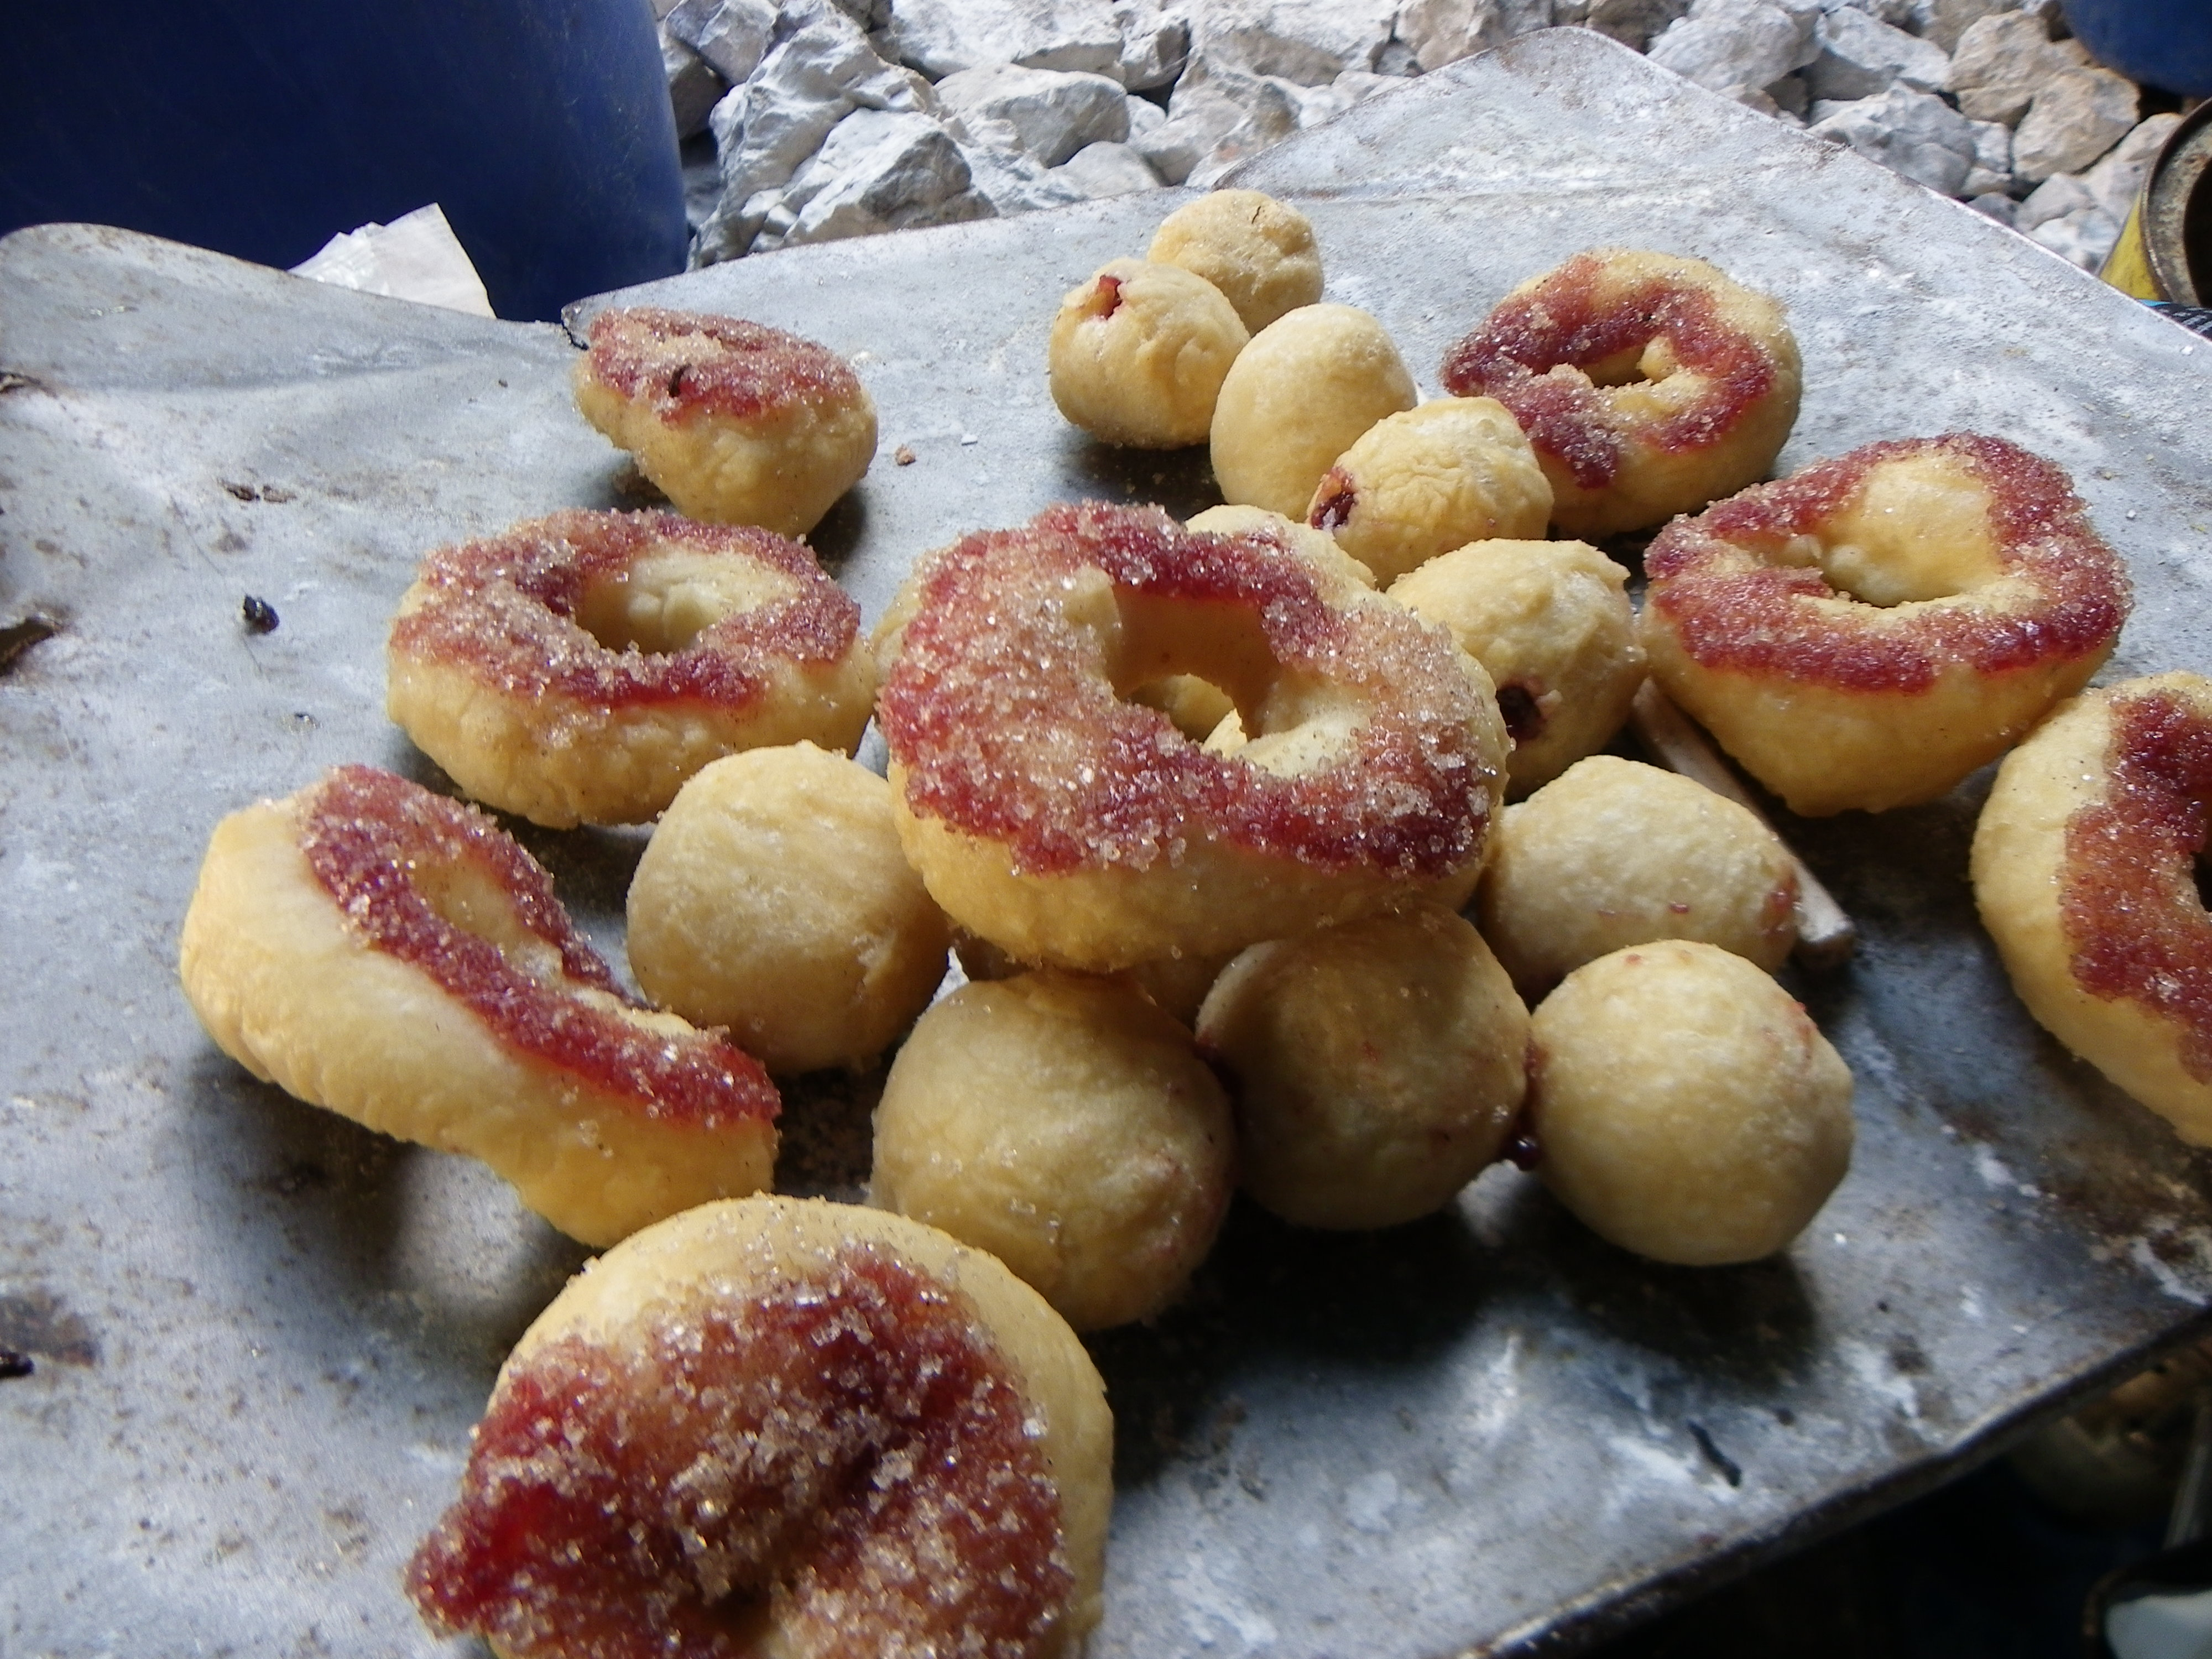
\includegraphics[width=\linewidth]{2012/alex_pitcher/rhys/2012-08-08-17.17.29-Rhys Tyers-Pentax X90-IMGP3388--orig.jpg}} 
 \caption{A hopefully delicious batch of donuts. \pic{Rhys Tyers}}
 \label{donuts}
\end{marginfigure}


Apart from the caving the whole trip was wonderful. The food in the \passage{Bivi} was always good and there was plenty of it. Making food was fun, I made quite a lot of donuts and failed to make nearly three cakes (incidentally some people like to eat half burnt/ half uncooked cake mix). Also the weather was generally superb which led to a lot of lazing on the mountainside reading.

It was an amazing experience and I can’t wait to go back next year.

\begin{pagefigure}
\checkoddpage \ifoddpage \forcerectofloat \else \forceversofloat \fi
   \centering
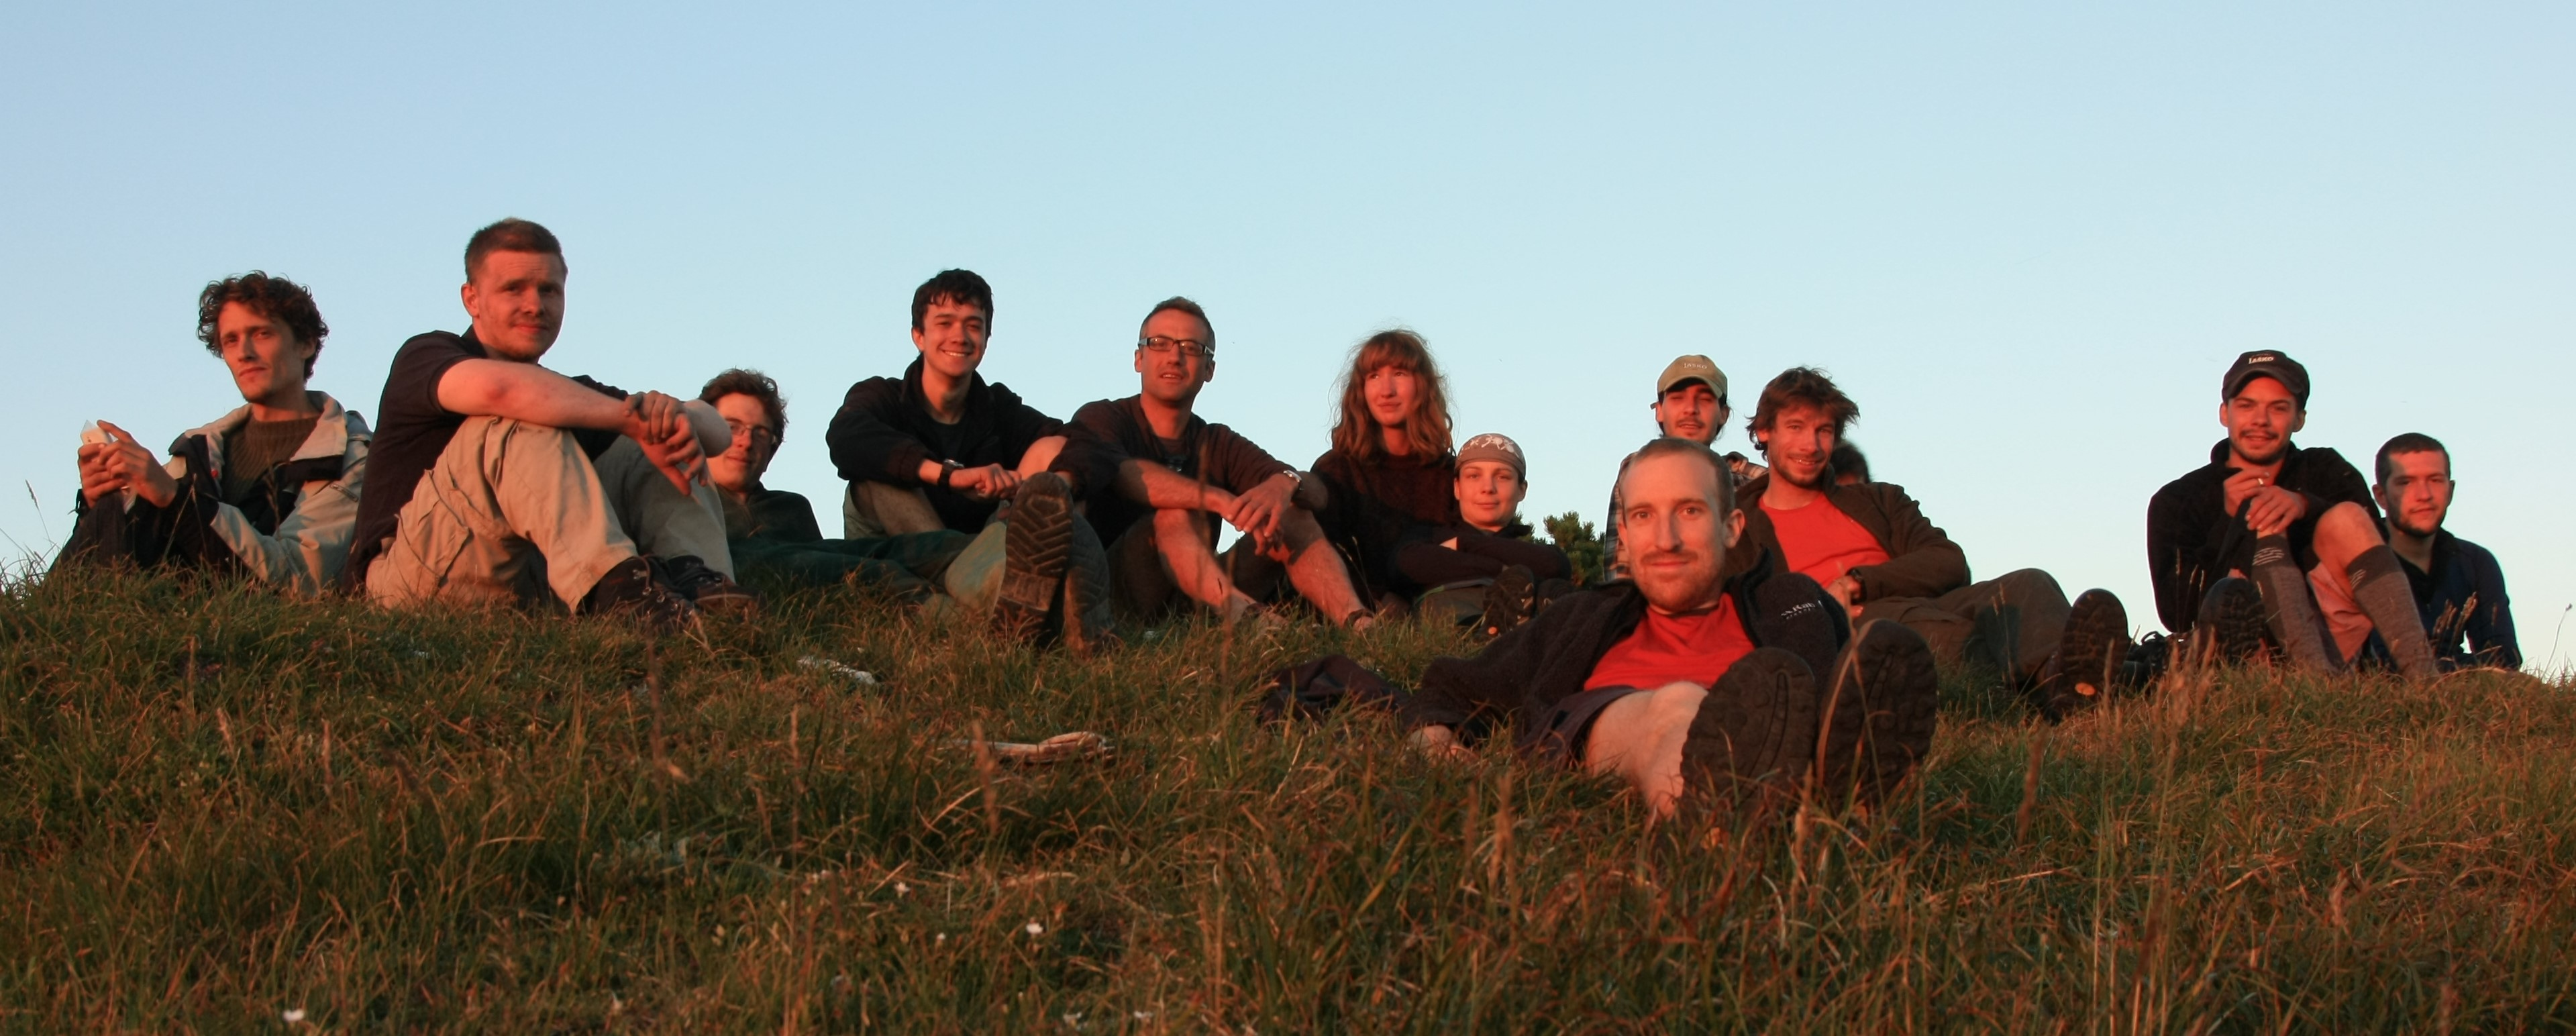
\includegraphics[width = \textwidth]{2012/alex_pitcher/rhys/2012-08-01-1123-GergelyAmbrus-IMG_2146--orig.jpg}
\caption{A mid-expo group shot. \textit{left to right} Jarvist Frost, William French, Oliver Myserscough, Rhys Tyers, Tetley, Kate Smith, Jana Carga, Andy Jurd (front), Izi Možir, Gergely Ambrus, Nejc Maver, Dan Greenwald. \pic{Gergely Ambrus}} \label{group sunset 2012}
\end{pagefigure}